\begin{figure*}
    \centering
    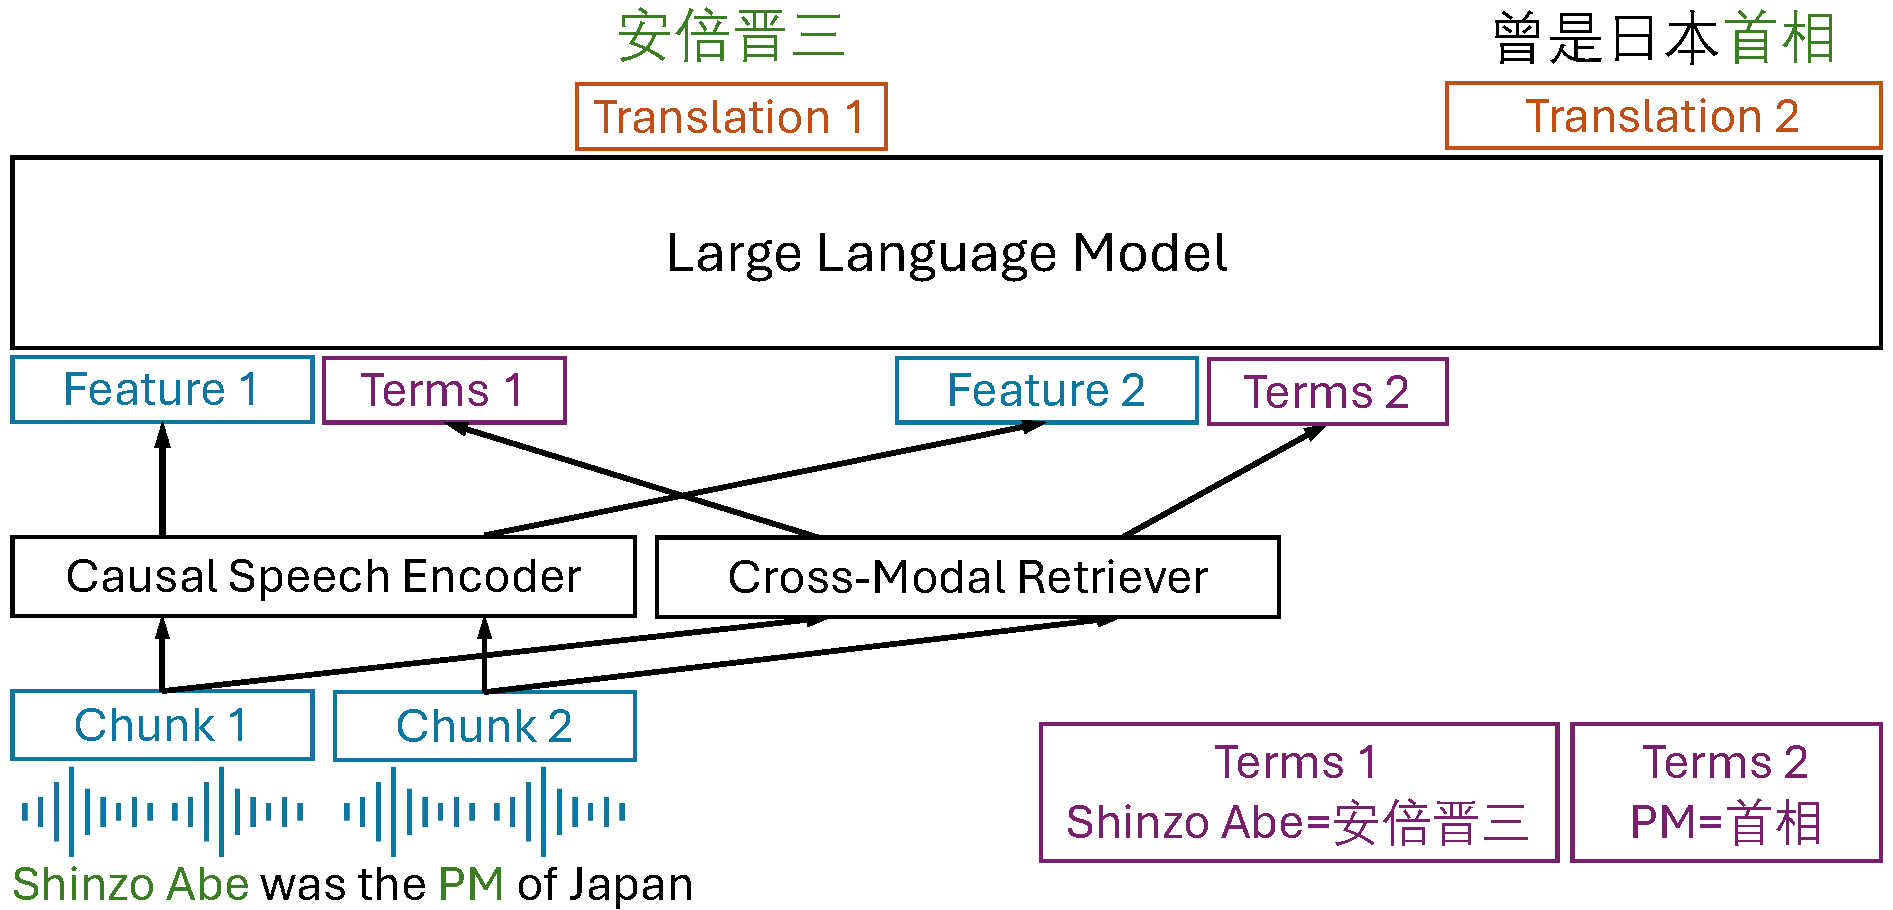
\includegraphics[width=0.9\linewidth]{latex/figures/overview.pdf}
    \caption{Overview of \method. \method interleaves speech chunks, retrieved terms, and translation outputs. For each incoming speech chunk, a causal speech encoder produces its feature representation, and a cross-modal retriever returns the corresponding terms. The retrieved terms are appended to the speech features and passed to the large language model, which decodes the next translation segment.}
    \label{fig:overview}
\end{figure*}

\section{Problem Formulation}
\label{sec:problem_formulation}

Let $\vs = (s_1, s_2, \dots, s_T) \in \mathbb{R}^T$ denote the source speech waveform, and let the glossary $\mathcal{G}=\{(e_j,e_j^\text{trans})\}_{k=1}^{|\mathcal{G}|}$, where $e_j$ is a term in the source language and $e_j^\text{trans}$ is its translation. At each step $i$, a fixed-duration speech chunk is received
\begin{align}
    \vs_i = \bigl(s_{i \cdot l + 1}, \dots, s_{(i+1) \cdot l}\bigr),
\end{align}
where $l$ is the chunk length.

Given the accumulated speech chunks $\vs_{1:i}$, the retriever $R_\phi$ selects a subset of relevant terminology entries
\begin{align}
    G_i = R_\phi(\vs_{1:i}, \mathcal{G}) \subseteq \mathcal{G} . \label{eqn:G_i}
\end{align}
Conditioned on the observed speech $\vs_{1:i}$, the previously generated translation tokens $\vy_{1:i-1}$, and the retrieved terminology context $G_{1:i}$, the model $\pi_\theta(\vs_{1:i}, \vy_{1:i-1}, G_{1:i})$ produces a partial translation $\vy_i$ at step $i$. The output $\vy_i = (y_1^i, \dots, y_{|\vy_i|}^i)$ may contain a variable number of tokens.

If $|\vy_i| = 0$, the model chooses to wait for additional speech input without emitting any translation. Otherwise, when $|\vy_i| > 0$, the model outputs a partial translation. All tokens in $\vy_i$ are assigned an identical delay of $i \cdot l$, corresponding to the elapsed time when the speech chunk $\vs_i$ becomes available.

Finally, translation quality and latency are evaluated with respect to the full source waveform $\vs$, the aggregated translation hypothesis $\vy$, the reference translation $\vy$, the source transcript $\vx$, and the delay associated with each generated token.

\section{Retrieval-Augmented Simultaneous Speech Translation}
\label{sec:method}

In this section, we first present an overview of RASST. We then describe the cross-modal retriever design and the training procedure that enables the Speech LLM to effectively leverage retrieved terms during simultaneous translation.

% Let $\vs=(s_1,s_2,\cdots,s_T)\in\mathbb{R}^T$ denote the source speech waveform and let $\mathcal{G}=\{(e_j,\tau_j)\}_{j=1}^{|\mathcal{G}|}$ be a bilingual glossary, where $e_j$ is a source-language term and $\tau_j$ is its target-language translation. 
% At each step $i$, a fixed-duration speech chunk is received
% \[
% \vs_i = \bigl(s_{i \cdot l + 1}, \dots, s_{(i+1) \cdot l}\bigr),
% \]
% where $l$ is the chunk length.
% At step $i$, the policy has access to the speech prefix $\mathbf{s}_{\le r_i}$ and the previously emitted target prefix $\hat{\mathbf{y}}_{<i}$, and it emits a possibly empty target segment $\hat{\mathbf{y}}_i$. Empty segments correspond to wait decisions; non-empty segments are appended to the final hypothesis $\hat{\mathbf{y}}$ with delay $r_i$.

% To ground terminology, we introduce a retriever $R_\phi$ that returns a step-local subset $\hat{\mathcal{G}}_i\subseteq\mathcal{G}$. The generator then models
% \begin{equation}
%   p_\theta(\hat{\mathbf{y}}_i \mid
%     \mathbf{s}_{\le r_i},
%     \hat{\mathbf{y}}_{<i},
%     \mathrm{format}(\hat{\mathcal{G}}_i)).
% \end{equation}
% The retrieved term map is evidence, not a hard constraint: the generator should use a term only when the audio context supports it.

\subsection{\method Overview}
\label{sec:method_overview}

Figure \ref{fig:overview} presents an overview of \method. We adopt the interleaving SST formulation of InfiniSST~\citep{ouyang-etal-2025-infinisst}, which alternates between incoming speech chunks and incremental translation outputs, and \method augments this with a retrieval step:
\begin{align}
\vy_i &\sim \mathrm{SpeechLLM}(\vs_1, G_1, \vy_1, \ldots, \vs_i, G_i).
\end{align}
After each chunk $\vs_i$ arrives, the retriever returns candidate terms $G_i$ likely to appear in it, and we append these terms along with their target-language translations to the chunk's representation. Conditioned on the speech context and the retrieved terms, the LLM then generates the next partial translation $\vy_i$.

\subsection{Cross-Modal Retriever}
\label{sec:retriever}

\paragraph{Architecture}
We adopt a dual-encoder architecture. For text, we use the pre-trained BGE-M3 encoder~\citep{bge-m3} to map each source-language term $e_j$ to a feature vector $\vg_j\in\mathbb{R}^d$. For speech, we use the Audio Transformer of Qwen3-Omni~\citep{yang2025qwen3technicalreport} followed by a linear projection to the same dimension $d$. Since terms are typically short, the speech encoder reads only the current chunk $\vs_i$ together with a look-back window of duration $t_{lb}$, rather than the full history $\vs_{1:i}$ as in Equation \ref{eqn:G_i}. We denote this input as $\vs_i'$ and the resulting features as $\vf_i\in\mathbb{R}^{m\times d}$, with $m$ as the number of frames in $\vs_i'$.

\begin{figure}
    \centering
    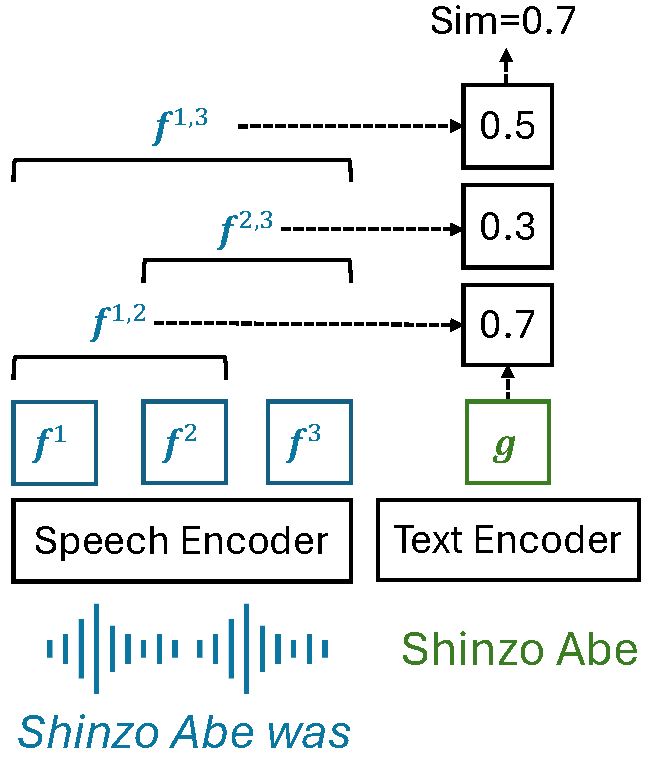
\includegraphics[width=0.8\linewidth]{latex/figures/multi_scale_retrieval.pdf}
    \caption{An example of multi-scale inference. The text term is encoded into a single feature vector $\vg$, while the speech context is encoded into frame features $\vf^1, \vf^2, \vf^3$. We enumerate all windows $(1,2), (2,3), (1,3)$ and compute the corresponding average-pooled features $\vf^{1,2}, \vf^{2,3}, \vf^{1,3}$. The likelihood that the term appears in the speech context is then the maximum cosine similarity between $\vg$ and any window feature.}
    \label{fig:multi_scale}
\end{figure}

\paragraph{Multi-Scale Inference}
Because terms vary in duration, representing the speech context with a single average-pooled vector loses information. Instead, we pool over windows at multiple scales. As shown in Figure \ref{fig:multi_scale}, given $\vf_i=(\vf_i^1,\vf_i^2,\ldots,\vf_i^m)$, for each window $1\leq u<v\leq m$ we compute
\begin{equation}
  \vf_i^{u,v} = \text{AvgPool}(\vf_i^u,\ldots,\vf_i^v)\in\mathbb{R}^d.
\end{equation}
The similarity between the speech $\vs_i'$ and a term $e_j$ is then the maximum cosine similarity over all windows:
\begin{equation}
  \text{Sim}(\vs_i',e_j)
  = \max_{1\leq u<v\leq m}
  \text{CosSim}(\vf_i^{u,v},\vg_j),
\end{equation}
and the retrieved terms are
\begin{align}
    G_i = \text{Top-}K_j\left(\text{Sim}(\vs_i',e_j)\right)\subseteq \mathcal{G}
\end{align}

In practice, we build a FAISS index~\citep{douze2024faiss} over the term vectors $\{\vg_j\}_{j=1}^{|\mathcal{G}|}$, then issue a Top-$K$ query for each window feature $\vf_i^{u,v}$, producing a candidate pool of size up to a multiple of $K$. We perform a second Top-$K$ selection over this pool by similarity score, keeping the highest score per term when duplicates occur, and finally discard any candidate whose similarity falls below a threshold $\tau$ to suppress noise.

\paragraph{Data Synthesis} \label{sec:retriever_data} Retriever training requires paired speech and terminology data $(\vs', e_\text{pos})$. Since terminology-rich speech corpora are scarce, we synthesize training data from two sources: existing ASR datasets and a terminology database.

For ASR data, we obtain word-level timestamps for each transcript using the Montreal Forced Aligner (MFA)\footnote{\url{https://github.com/MontrealCorpusTools/Montreal-Forced-Aligner}}, then extract noun phrases as candidate terms using spaCy\footnote{\url{https://spacy.io/} and  \texttt{en\_core\_web\_trf} model} and normalize their surface forms. We use noun phrases because most domain-specific terminology takes this form and they are abundant in standard transcripts. For each term, we carve out a speech context $\vs'$ of variable duration surrounding it, which gives the retriever flexibility across context lengths at inference time.

For each term in the terminology database, we prompt Gemini-2.5-Flash\footnote{\url{https://ai.google.dev/gemini-api/docs/models/gemini-2.5-flash}} to generate several sentences containing the term and synthesize the speech with CosyVoice 3~\citep{du2025cosyvoice}. The resulting speech is then processed by the same MFA pipeline as the ASR data.

\paragraph{Training} 
Given paired data $(\vs', e_\text{pos})$, we train the retriever with the InfoNCE loss~\citep{oord2019representationlearningcontrastivepredictive}. In addition to in-batch negatives, we mine hard negatives by using the retriever checkpoint, which is updated every 50 training steps, to retrieve the Top-$N$ most similar terms from the entire training set for each positive $e_\text{pos}$.
Let $E_\text{neg}$ be the negative set and $E_\text{all} = \{e_\text{pos}\} \cup E_\text{neg}$. The retriever loss $\mathcal{L}_{\mathrm{retriever}}$ is then \begin{equation} 
-\log \frac{ \exp(\text{Sim}(\vs_i',e_\text{pos})/\gamma) }{ \sum_{e\in E_\text{all}} \exp(\text{Sim}(\vs_i',e)/\gamma) }, 
\end{equation} where $\gamma$ is the temperature. 
Since the timestamp of $e_\text{pos}$ within $\vs'$ is known during training through MFA, we bypass the maximum over windows in $\text{Sim}(\cdot)$ and instead set $(u, v)$ to be the smallest window enclosing $e_\text{pos}$.


\subsection{Speech LLM Training}
\label{sec:rag_sst_generator}

To teach the Speech LLM to effectively use the retrieved terms $G_i
$ during simultaneous translation, we synthesize a corresponding training corpus. Given the speech chunks $\vs_{1:i}$, we follow InfiniSST's procedure to produce the translation segments $\vy_{1:i}$. The remaining piece beyond InfiniSST is the retrieved terms $G_{1:i}$. A naive approach is to reuse the noun-phrase terms from retriever training and always populate $G_i$ with the ground-truth term. This, however, would leave the model brittle to retriever mistakes at inference time. To reduce this training–inference mismatch, we build a glossary over all noun phrases in the training set and run the cross-modal retriever from Section~\ref{sec:retriever} on every speech chunk. Then we add the retrieved distractors in $G_i$ alongside the ground-truth term. The Speech LLM thus learns to translate in the presence of realistic retriever noise.

A training example is shown in Figure \ref{fig:train_prompt_visual}. We wrap the ground-truth term's translation in a \texttt{\textless term\textgreater\ldots\textless/term\textgreater} tag, encouraging the Speech LLM to copy ground-truth term translations directly from $G_i$. We fine-tune with a standard cross-entropy objective applied only to translation tokens $\vy$. Because translations naturally lag behind speech in the training data, the model also receives implicit supervision for \emph{timing}: it observes when a term appears in the speech context and when its translation appears later in the target sequence.